\documentclass[letterpaper]{article}
\usepackage{proceed2e}
\usepackage[margin=1in]{geometry}
\usepackage{mathtools}
\usepackage{amsfonts}
\usepackage{amsthm}
\usepackage{subfig}
\usepackage{hyperref}

\usepackage{times}
\usepackage{float}

\usepackage{natbib}

\usepackage{bbm}

\newtheorem{theorem}{Theorem}
\newtheorem{lemma}{Lemma}

\allowdisplaybreaks

\title{Uncertainty propagation in deep neural networks for sparse coding}

\author{} % LEAVE BLANK FOR ORIGINAL SUBMISSION.
          % UAI  reviewing is double-blind.

% The author names and affiliations should appear only in the accepted paper.
%
%\author{ {\bf Harry Q.~Bovik\thanks{Footnote for author to give an
%alternate address.}} \\
%Computer Science Dept. \\
%Cranberry University\\
%Pittsburgh, PA 15213 \\
%\And
%{\bf Coauthor}  \\
%Affiliation          \\
%Address \\
%\And
%{\bf Coauthor}   \\
%Affiliation \\
%Address    \\
%(if needed)\\
%}

%\author{ {\bf Danil Kuzin} \\
%\And
%{\bf Olga Isupova}  \\
%\And
%{\bf Lyudmila Mihaylova}   \\
%}

\begin{document}

\maketitle

\begin{abstract}
In the Bayesian neural network framework prior distributions are imposed on weights of a network and a posterior distribution of an output is inferred, rather than a point prediction provided by conventional neural networks. Therefore, Bayesian neural networks estimate both an output for a test data and uncertainty of this prediction. Uncertainty of the prediction is a result of propagating weight uncertainty through layers of a network. We propose a novel method of propagating uncertainty through the soft thresholding nonlinearity. The method expands the area of Bayesian neural networks and enables the soft thresholding nonlinearity to be included in Bayesian deep neural networks for the first time. As an example we design a Bayesian Learned Iterative Shrinkage-Thresdholding Algorithm (Bayesian \textsc{lista}) network. We develop a highly efficient posterior inference algorithm based on probabilistic backpropagation. A series of experiments on sparse coding shows that the proposed framework provide both accurate predictions and quantified estimates of uncertainty in these predictions.
\end{abstract}

\section{\uppercase{Introduction}}
Though the idea of Bayesian learning in neural networks is not new \citep{neal2012bayesian}, it has regained its attention recently with the development of distributed approximate inference techniques \citep{li2015stochastic, hoffman2013stochastic}  and general boost in popularity of deep learning. In some spheres, such as self-driving cars or healthcare, uncertainty estimates are very important and Bayesian learning allows to obtain them. 

In general, when distributions are included in a network, Bayesian inference complexity scales exponentially with the number of layers. Thus, it is infeasible to apply conventional Bayesian inference algorithms for deep neural networks. Nevertheless, recently several techniques have been proposed to handle specific types of neural networks. For example, feed-forward networks with rectified linear units nonlinearity~\citep{hernandez2015probabilistic}, networks with discrete distributions~\citep{soudry2014expectation}, recurrent networks~\citep{mcdermott2017bayesian}. 

There are currently two approaches in Bayesian neural networks: explicit distributions of weights can be included in a network \citep{hernandez2015probabilistic, ranganath2015deep}, or dropout can be interpreted as an element introducing uncertainty \citep{gal2016dropout}. In this paper we use the first way and impose distributions on weights to obtain posterior estimates of weights and predictions with uncertainty estimated.

Sparse coding can be viewed as a linear regression problem with the additional assumption that many of the basis representation coefficients should be zeros. They arise in different applications, such as compressive sensing~\citep{candes2008introduction}, image and video processing~\citep{mairal2014sparse}, neuroscience~\citep{baillet1997bayesian, jas2017learning}. 

Neural networks address the sparse coding problem with the soft thresholding nonlinearity, that shifts current estimates towards zero \citep{gregor2010learning}. In this paper we propose a method to propagate uncertainty through the soft thresholding nonlinearity. At every layer the current distribution of the target vector is represented as a spike and slab distribution \citep{mitchell1988bayesian}. We show that it can be effectively combined with Gaussian weights of dense layers. The distribution of the target vector propagated through a dense layer and soft thresholding nonlinearity can then be closely approximated with a distribution from the same family.

The proposed method of uncertainty propagation for the soft thresholding nonlinearity allows us to derive the gradients of the logarithms of normalisation constants, which can be used to update weights distribution. We then develop a highly efficient Bayesian inference algorithm based on the probabilistic backpropagation paradigm while significantly expanding it.

The main contributions of this paper can be summarised~as: 
\begin{itemize}
\item for the first time we propose a method for uncertainty propagation through the soft thresholding nonlinearity for a Bayesian neural network;
\item we develop efficient posterior inference for weights and outputs of neural networks with the soft thresholding nonlinearity;
\item we design a novel Bayesian neural network for sparse coding.
\end{itemize}

The paper is organised as following: first, we review neural networks for sparse coding in section \ref{sec:nn_sc} and present a novel Bayesian neural network in section \ref{sec:bayesian_lista}. We then describe uncertainty propagation to obtain the spike and slab distribution for an output of a network in section \ref{sec:fprop} and how probabilistic backpropagation is organised to update distributions of weights in section \ref{sec:backpropagation}. After that, we show the experimental results of the algorithm in section \ref{sec:experiments} and finish with discussion and conclusions in sections \ref{sec:discussion} and \ref{sec:conclusions}.

\section{\uppercase{Neural networks for sparse coding}}
\label{sec:nn_sc}
The sparse coding problem is the linear regression with the assumption of sparse weights
\begin{equation}
\label{eq:regression_problem}
\mathbf{y} = \mathbf{X}\boldsymbol\beta + \varepsilon
\end{equation}
where $\mathbf{y} \in \mathbb{R}^K$ is the observation, $\mathbf{X} \in \mathbb{R}^{K \times D}$ is the design matrix, $\boldsymbol\beta \in \mathbb{R}^D$ is the unknown vector of weight with many elements $\beta_d$ equal to zero. $\varepsilon \in \mathbb{R}^K$ is the independent Gaussian noise.

One of the popular families of the sparse coding algorithms is the iterative shrinkage algorithms, and notably the Iterative Shrinkage and Thresholding Algorithm(\textsc{ista}) \citep{daubechies2004iterative}. It iteratively obtains the new approximation of the coefficient vector $\widehat{\boldsymbol\beta}_l$ at the iteration $l$ as the linear transformation of the input $\mathbf{y}$ with previous approximation $\widehat{\boldsymbol\beta}_{l-1}$ and then propagates the new approximation through the soft thresholding function $h_\lambda(\cdot)$
\begin{equation}
h_\lambda(v) = \text{sgn}(v) \max(|v| - \lambda, 0)
\end{equation}
where $\lambda$ is a shrinkage parameter.
The linear transformation is
\begin{equation}
\widehat{\boldsymbol\beta}_l = \mathbf{W}\mathbf{y} + \mathbf{S}_l\widehat{\boldsymbol\beta}_{l-1}
\end{equation}
with weights $\mathbf{W} = \mathbf{X}^\top / E$, $E$ - upper bound on the largest eigenvalue of $\mathbf{X}^\top\mathbf{X}$ and $\mathbf{S} = \mathbf{I}_{D \times D} - \mathbf{W}\mathbf{X}$ ($\mathbf{I}_{D \times D}$ is the identity matrix of size $D$).

The Learned \textsc{ista} (\textsc{lista}) \citep{gregor2010learning} algorithm allows to learn the values of matrices $\mathbf{W}$, $\mathbf{S}$ based on set of pairs $\{\mathbf{Y}, \mathbf{B}\}=\{\mathbf{y}^{(n)}, \boldsymbol\beta^{(n)}\}_{n=1}^N$, where $N$ is the number of these pairs. To achieve this, \textsc{ista} algorithm is limited with the fixed amount of iterations, $L$ and interpreted as a recurrent neural network. Overall, it has the following scheme of predicting a coefficient vector $\boldsymbol\beta$ for an observation $\mathbf{y}$
\begin{align}
\label{eq:first_layer}
&\mathbf{b} = \mathbf{W}\mathbf{y}\\
\label{eq:thr_first}
&\widehat{\boldsymbol\beta}_0 = h_\lambda(\mathbf{b}) \\
&\text{for } l=1:L\\
\label{eq:l_dense_layer}
	&\quad \mathbf{c}_l = \mathbf{b} + \mathbf{S}\widehat{\boldsymbol\beta}_{l-1} \\
\label{eq:l_thr}
	&\quad \widehat{\boldsymbol\beta}_{l} = h_\lambda(\mathbf{c}_l) \\
& \widehat{\boldsymbol\beta} = \widehat{\boldsymbol\beta}_{L}
\end{align}

Matrices $\mathbf{W}$, $\mathbf{S}$ are the parameters that are initialised as in \textsc{ista} and then updated with the backpropagation algorithm. Vectors $\mathbf{c}_l$, $\mathbf{b}$ are intermediate vectors that describe forward propagation. 

\section{\uppercase{Bayesian neural network for sparse coding}}
\label{sec:bayesian_lista}

This section presents the proposed Bayesian neural network for sparse coding. To formulate the Bayesian version of \textsc{lista} we impose the prior distributions on the unknown weights
\begin{subequations}
\label{eq:ws}
\begin{align}
&p(\mathbf{W}) = \prod_{d=1}^D\prod_{k=1}^K \mathcal{N}(w_{ij} | 0, \eta^{-1}), \\
&p(\mathbf{S}) = \prod_{d'=1}^D\prod_{d''=1}^D \mathcal{N}(s_{d'd''} | 0, \eta^{-1}),
\end{align}
\end{subequations}
where $w_{ij}$ is a component of the matrix $\mathbf{W}$, $s_{d'd''}$ is a component of the matrix $\mathbf{S}$, $\eta$ is the precision of the Gaussian distribution.
The likelihood of $\mathbf{B}$ is defined as 
\begin{align}
p(&\mathbf{B}| \mathbf{Y}, \mathbf{W}, \mathbf{S}, \gamma, \lambda) \nonumber \\
\label{eq:likelihood}
= &\prod_{n=1}^N\prod_{d=1}^D\mathcal{N}(\beta_d^{(n)}; [f(\mathbf{y^{(n)}}; \mathbf{W}, \mathbf{S}, \lambda)]_d, \gamma^{-1}),
\end{align}
where $[\cdot]_d$ denotes the d-th component of a vector, $f(\mathbf{y}^{(n)}; \mathbf{W}, \mathbf{S}, \lambda)$ is the output of the Bayesian \textsc{lista} neural network, $\gamma$ is the precision of the Gaussian distribution.
The prior of the introduced Gaussian precisions are set to the Gamma distribution with parameters $a^{\cdot}$ and $b^{\cdot}$:
\begin{subequations}
\label{eq:gamma_eta}
\begin{align}
&p(\gamma) = \text{Gam}\left(\gamma; a^{\gamma}, b^{\gamma}\right), \\
&p(\eta) = \text{Gam}\left(\eta; 	a^{\eta}, b^{\eta}\right)
\end{align}
\end{subequations}

The posterior distribution is then
\begin{align}
p(&\mathbf{W}, \mathbf{S}, \gamma, \eta | \mathbf{B}, \mathbf{Y}, \lambda) \nonumber \\
\label{eq:posterior}
= & \frac{p(\mathbf{B} | \mathbf{Y}, \mathbf{W},  \mathbf{S}, \gamma, \lambda) p(\mathbf{W} | \eta )p(\mathbf{S} | \eta) p(\eta) p(\gamma)}{p(\mathbf{B} | \mathbf{Y}, \lambda)}
\end{align}
The shrinkage parameter $\lambda$ is a hyperparameter of the model.

\section{\uppercase{Uncertainty propagation through soft thresholding}}
\label{sec:fprop}
For every layer of the Baysian \textsc{lista} we assume that $\widehat{\boldsymbol\beta}_{l-1}$ has the spike and slab distribution with parameters: $\boldsymbol\omega$ is a probability of a spike, $\mathbf{m}$ is a mean of a slab Gaussian distribution, and $\mathbf{v}$ is a variance of the slab distribution:
\begin{equation}
[\widehat{\boldsymbol\beta}_{l-1}]_d \sim \omega_d \delta_0 + (1 - \omega_d)\mathcal{N}(m_d, v_d),
\end{equation}
where $\omega_d$, $m_d$, and $v_d$ are components of vectors $\boldsymbol\omega$, $\mathbf{m}$, and $\mathbf{v}$, respectively, $\delta_0$ is the delta-function that represents a spike. 
We initialise $\widehat{\boldsymbol\beta}_{0}$ with the spike and slab distribution with parameters $\boldsymbol\omega = \mathbf{0}$, $\mathbf{m} = \mathbf{0}$, and $\mathbf{v} = \mathbf{1}$. 

Later in this section, we show that the output $\widehat{\boldsymbol\beta}_l$ of the next layer can be approximated with a spike and slab distribution and, therefore, it maintains the same family of distributions. This leads to the proposed probabilistic backpropagation algorithm that is presented in Section~\ref{sec:backpropagation}. We now describe how to propagate uncertainty through the layers of the Bayesian \textsc{lista} step by step stating meanwhile theoretical facts required for the method.

\subsection{\uppercase{Initialisation dense layer}}
The first step in the Bayesian \textsc{lista} is (\ref{eq:first_layer}). The matrix $\mathbf{W}$ consists of Gaussian-distributed components and $y$ is a deterministic vector.

 \begin{lemma}[Product of Gaussian matrix and constant vector]
 \label{thm:matrix_const}
Let $\mathbf{W} \in \mathbb{R}^{D \times K}$ be a matrix of independent Gaussian-distributed random variables: $w_{dk} \sim \mathcal{N}(m^w_{dk}, v^w_{dk})$, and $\mathbf{y} \in \mathbb{R}^K$ be a constant vector. Then their product $\mathbf{W} \mathbf{y}$ is a vector $\mathbf{b} \in \mathbb{R}^{D}$ of random variables $b_d \sim \mathcal{N}(m^b_d, w^b_d)$, where 
\begin{subequations}
\begin{align}
m^b_d &= \sum_{k=1}^Ky_k m^w_{dk}, \\
w^b_d &= \sum_{k=1}^Ky_k^2v^w_{dk}.
 \end{align}
\end{subequations}
 
 \end{lemma}
 \begin{proof}
 	The statement follows from the property that the family of normal distributions is closed under linear transformations.
 \end{proof}
 
According to Lemma~\ref{thm:matrix_const}, $\mathbf{b}$ in~(\ref{eq:first_layer}) is a vector of Gaussian-distributed components.


\subsection{\uppercase{Soft thresholding nonlinearity}}
At the second step (\ref{eq:thr_first}) of the Bayesian \textsc{lista} the Gaussian vector $\mathbf{b}$ is taken as an input of the soft thresholding function.

When a Gaussian-distributed random variable $x \sim \mathcal{N}(x; m, v)$ is propagated through the soft thresholding function: $x^* = h_{\lambda}(x)$ the probability mass of a resulting random variable $x^*$ is split into two parts. The values of $x$ from the interval $[-\lambda, \lambda]$ are converted to $0$ by the soft thresholding operator. Therefore, the probability mass of the original distribution that lies in $[-\lambda, \lambda]$ is squeezed into the probability of $x^*$ being zero. The values of $x$ from outside of the $[-\lambda, \lambda]$ interval are shifted towards $0$. Therefore, the distribution of $x^* \neq 0$ represents the tails of the original Gaussian distribution.
 
\begin{lemma}[Propagation of a Gaussian distribution through soft thresholding]
\label{thm:soft_thresholding}
The distribution of $x^*$ can be parametrised by the probability of being zero, $\omega^*$, the mean $m^*$ and the variance $v^*$ of the truncated Gaussian distribution.
\end{lemma}
\begin{proof}

The probability of a zero $\omega^*$ equals to the probability mass of the original distribution from the interval $[-\lambda, \lambda]$
\begin{align}
\begin{split}
\omega^* &= \mathbb{P}(x^*=0) = \mathbb{P}(x \in [-\lambda, \lambda]) \\
&= \Phi\left(\frac{\lambda-m}{\sqrt{v}}\right) - \Phi\left(\frac{-\lambda-m}{\sqrt{v}}\right). 
\end{split}
\end{align}
where $\Phi(\cdot)$ is the standard Gaussian cumulative distribution function. 

The soft thresholding function shifts elements that are greater than $\lambda$  or less than $-\lambda$ towards $0$. Let $\psi(\cdot)$ denote the density of the soft thresholded distribution on $x^* \neq 0$, $\phi(\cdot)$ denote the density of the original Gaussian distribution on $x$. Then the first moment of $x^* \neq 0$ is:

\begin{align}
\label{eq:thr_first_moment}
\begin{split}
m^* &= \int_{-\infty}^{+\infty}x\psi(x)dx= \int_{-\infty}^{0}x\phi(x-\lambda)dx \\
&{} + \int_{0}^{+\infty}x\phi(x+\lambda)dx,
\end{split}
\end{align}
where
\begin{align}
&\int_{-\infty}^{0}x\phi(x-\lambda)dx = -\frac{\sqrt{v}}{\sqrt{2\pi}} \exp\left\{\frac{-(\lambda+m)^2}{2v}\right\} \nonumber\\
&{} + (\lambda+m)\Phi\left(-\frac{\lambda+m}{\sqrt{v}}\right)\\
&\int_{0}^{+\infty}x\phi(x+\lambda)dx = \frac{\sqrt{v}}{\sqrt{2\pi}} \exp\left\{\frac{-(m - \lambda)^2}{2v}\right\}\nonumber\\
& + (m - \lambda)\left(1 - \Phi\left(-\frac{\lambda-m}{\sqrt{v}}\right)\right)
\end{align}

The second moment of $x^* \neq 0$ is given as
\begin{align}
\label{eq:thr_second_moment}
\begin{split}
s &= \int_{-\infty}^{+\infty}x^2\psi(x)dx = \int_{-\infty}^{0}x^2\phi(x-\lambda)dx \\
&{}+ \int_{0}^{+\infty}x^2\phi(x+\lambda)dx,
\end{split}
\end{align}
where
\begin{align}
\begin{split}
&\int_{-\infty}^{0}x^2\phi(x-\lambda)dx = \\
&-\frac{\sqrt{v}}{\sqrt{2\pi}} (\lambda+m)\exp\left\{\frac{-(\lambda+m)^2}{2v}\right\}\\
& + (\sigma^2 + (\lambda+m)^2)\Phi\left(-\frac{\lambda+m}{\sqrt{v}}\right)
\end{split}\\
\begin{split}
&\int_{0}^{+\infty}x^2\phi(x+\lambda)dx = \\
&\frac{\sqrt{v}}{\sqrt{2\pi}} (m - \lambda)\exp\left\{\frac{-(m - \lambda)^2}{2v}\right\}\\
& + (\sigma^2 + (m - \lambda)^2)\left(1 - \Phi\left(\frac{\lambda -m}{\sqrt{v}}\right)\right)
\end{split}
\end{align}

The resulting variance is then
\begin{equation}
v^* = s- (m^*)^2
\end{equation}
\end{proof}

Based on the results of Lemma~\ref{thm:soft_thresholding} we approximate the distribution of $\widehat{\boldsymbol\beta}_0$ from (\ref{eq:thr_first}) with a spike and slab distribution with parameters derived in the lemma: spike probability $\omega$ is equal to $\omega^*$, slab mean $m$ and variance $v$ are set to the corresponding parameters of the truncated Gaussian $m^*$ and $v^*$.

\subsection{\uppercase{Main layers}}
The distributions of the inputs at the step (\ref{eq:l_dense_layer}) of the Baysian \textsc{lista} for each $l$ are: the vector $\mathbf{b}$ and matrix $\mathbf{S}$ consist of Gaussian-distributed components and $\widehat{\boldsymbol\beta}_{l-1}$ is a vector of the spike and slab random variables.

In order to determine the distribution of the output $\mathbf{c}_l$ we first formulate two lemmas.

\begin{lemma}[Moments of a spike and slab distribution]
\label{thm:moments_spsl}
Let a random variable $\xi$ have a spike and slab distribution with probability of spike $\omega$, slab mean $m$ and slab variance $v$. Then its moments are
\begin{subequations}
\begin{align}
\mathbb{E}\xi &= (1-\omega)m \\
\operatorname{Var}\xi & = (1-\omega)(v + \omega m^2)
\end{align}
\end{subequations}
\end{lemma}

\begin{proof}
\begin{align*}
\begin{split}
\mathbb{E}\xi &= \int x \big(\omega \delta_0(x) + (1 - \omega)\mathcal{N}(x; m, v)\big)dx \\
& = \omega \int x \delta_0(x)dx + (1 - \omega)\int x \mathcal{N}(x; m, v)dx \\
& = (1-\omega)m \\
\mathbb{E}\xi^2 &= \int x^2 \big(\omega \delta_0(x) + (1 - \omega)\mathcal{N}(x; m, v)\big)dx \\
& = \omega \int x^2 \delta_0(x)dx + (1 - \omega)\int x^2 \mathcal{N}(x; m, v)dx \\
& = (1-\omega)(v + m^2) \\
\operatorname{Var}\xi &= \mathbb{E}\xi^2 - \left(\mathbb{E}\xi\right)^2 = (1-\omega)(v + \omega m^2)
\end{split}
\end{align*}
\end{proof}

\begin{lemma}[Product of a Gaussian matrix and a spike and slab vector]
  \label{thm:matrix_vector}
Let $\mathbf{S} \in \mathbb{R}^{D \times D}$ be a matrix of independent Gaussian-distributed random variables: $s_{d'd''} \sim \mathcal{N}(m^s_{d'd''}, v^s_{d'd''})$, and $\widehat{\boldsymbol\beta }\in \mathbb{R}^D$ be a vector with spike-and-slab distributed variables: $\widehat{\beta}_d \sim \omega_d \delta_0 + (1 - \omega_d)\mathcal{N}(m_d, v_d)$. The components of the matrix $\mathbf{S}$ and the vector $\widehat{\boldsymbol\beta}$ are mutual independent. Let $\mathbf{e} \in \mathbb{R}^{D}$ denote the product $\mathbf{S} \widehat{\boldsymbol\beta}$. Then the marginal mean and variance of elements $e_d$ of the vector $\mathbf{e}$ are:
\begin{subequations}
\begin{align}
 \mathbb{E}e_d &= \sum_{d'=1}^D m^s_{dd'}(1-\omega_{d'})m_{d'}, \\
 \begin{split}
 \operatorname{Var}e_d &= \sum_{d'=1}^D [(m^s_{dd'})^2(1-\omega_{d'})^2v_{d'} \\
 & {}+ (1-\omega_{d'})^2(m_{d'})^2v^s_{dd'} + v^s_{dd'}(1-\omega_{d'})^2v_{d'}].
 \end{split}
 \end{align}
\end{subequations}
 \end{lemma}
 \begin{proof}
\begin{flalign*}
	\mathbb{E}e_d &= \sum_{d'=1}^D \mathbb{E}[s_{dd'}\widehat{\beta}_{d'}]  = \sum_{d'=1}^D m^s_{dd'}\mathbb{E}\widehat{\beta}_{d'}\\
	\operatorname{Var}e_d &= \sum_{d'=1}^D \operatorname{Var}[s_{dd'}\widehat{\beta}_{d'}] = \sum_{d'=1}^D [(\mathbb{E}s_{dd'})^2 \operatorname{Var}\widehat{\beta}_{d'} \\
	&{}+ (\mathbb{E}\widehat{\beta}_{d'})^2 \operatorname{Var}s_{dd'} + \operatorname{Var}\widehat{\beta}_{d'} \operatorname{Var}s_{dd'}]
\end{flalign*}
where $\mathbb{E}\widehat{\beta}_{d'}$, $\operatorname{Var}\widehat{\beta}_{d'}$ are computed according to lemma~\ref{thm:moments_spsl}.
 \end{proof}
 
Let $\mathbf{e}_l = \mathbf{S}\widehat{\boldsymbol\beta}_{l-1}$ at the step (\ref{eq:l_dense_layer}) of the Baysian \textsc{lista}. We assume that $\mathbf{S}$ and $\widehat{\boldsymbol\beta}_{l-1}$ are mutually independent. Then according to the Central Limit Theorem $[ \mathbf{e}_l ]_d$ can be approximated as a Gaussian-distributed variable when $D$ is sufficiently large. The parameters of the of the approximating Gaussian distribution are set to the marginal mean and variance given in Lemma~\ref{thm:matrix_vector}. The quality of this approximation is discussed in section \ref{sec:approx_quality}.

The output $\mathbf{c}_l$ at the step (\ref{eq:l_dense_layer}) is then represented as a sum of two Gaussian-distributed vectors: $\mathbf{b}$ and $\mathbf{e}_l$


\begin{lemma}[Sum of Gaussian vectors]
\label{thm:sum_vectors}
If $\mathbf{b} \in \mathbb{R}^{D}$ and $\mathbf{e} \in \mathbb{R}^{D}$ are both vectors of independent Gaussian-distributed random variables: $b_{d} \sim \mathcal{N}(m^b_{d}, v^b_{d})$, $e_{d} \sim \mathcal{N}(m^e_{d}, v^e_{d})$ then their sum $\mathbf{c} = \mathbf{b} + \mathbf{e}$ is a vector of independent Gaussian-distributed random variables $c_{d} \sim \mathcal{N}(m^c_{d}, v^c_{d})$ with 
\begin{subequations}
\begin{align}
m^c_{d} &= m^b_{d} + m^e_{d}, \\
v^c_{d} &= v^b_{d} + v^e_{d}.
 \end{align}
\end{subequations}
\end{lemma}
\begin{proof}
Based on properties of Gaussian distributions.
\end{proof}

Therefore, $\mathbf{c}_l$ is a vector of Gaussian-distributed components, which parameters can be found according to Lemma~\ref{thm:sum_vectors}.

Then $\widehat{\boldsymbol\beta}_{l}$ at the step (\ref{eq:l_thr}) of the Baysian \textsc{lista} is the result of soft thresholding of a Gaussian distribution, which is approximated with the spike and slab distribution,  similar to the step (\ref{eq:thr_first}). 

\subsection{\uppercase{Bayesian lista forward propagation}}
We have covered all steps of the Bayesian \textsc{lista} and derived distributions for outputs of these steps. Now we can formulate the main result of this section that describes how the proposed uncertainty propagation works.

\begin{enumerate}
	\item $\mathbf{b} = \mathbf{W}\mathbf{y}$ is the Gaussian distribution with parameters computed according to lemma \ref{thm:matrix_const};
	\item $\mathbf{e}_l = \mathbf{S}\widehat{\boldsymbol\beta}_{l-1}$ is approximated with the Gaussian distribution, which parameters are computed according to lemma \ref{thm:matrix_vector};
	\item $\mathbf{c} = \mathbf{b} + \mathbf{e}$ is the Gaussian distribution with parameters computed according to lemma \ref{thm:sum_vectors};
	\item $\widehat{\boldsymbol\beta}_{l} = h_\lambda(\mathbf{c})$ is approximated with the spike and slab distribution, which parameters are computed according to lemma \ref{thm:soft_thresholding}.
\end{enumerate}


\subsection{\uppercase{Approximation quality}}
\label{sec:approx_quality}
We have used two approximations in forward propagation of uncertainty. First, in lemma \ref{thm:matrix_vector} a Gaussian matrix is multiplied by a spike and slab vector and their product is approximated with the Gaussian distribution. Second, in lemma \ref{thm:soft_thresholding} the result of soft thresholding of a Gaussian vector is approximated with the spike and slab distribution. In this section we demonstrate that these approximations are close to the real distributions.

Figure \ref{fig:d_testing} demonstrates the comparison of the sampled distribution and approximated distribution for lemma \ref{thm:matrix_vector}. For sampled distribution, $10000$ values were sampled from the Gaussian matrix and the spike and slab vector and their product is computed, then one of the dimensionalities is plotted. The approximated distribution is computed according to lemma \ref{thm:matrix_vector}.

Figure \ref{fig:z_new_testing} demonstrates the comparison of the sampled distribution and approximated distribution for lemma \ref{thm:soft_thresholding}. For sampled distribution, $10000$ values are sampled from the Gaussian vector and propagated through soft thresholding, then one of the dimensionalities is plotted. The approximated distribution is computed according to lemma \ref{thm:soft_thresholding}.
\begin{figure}[t]
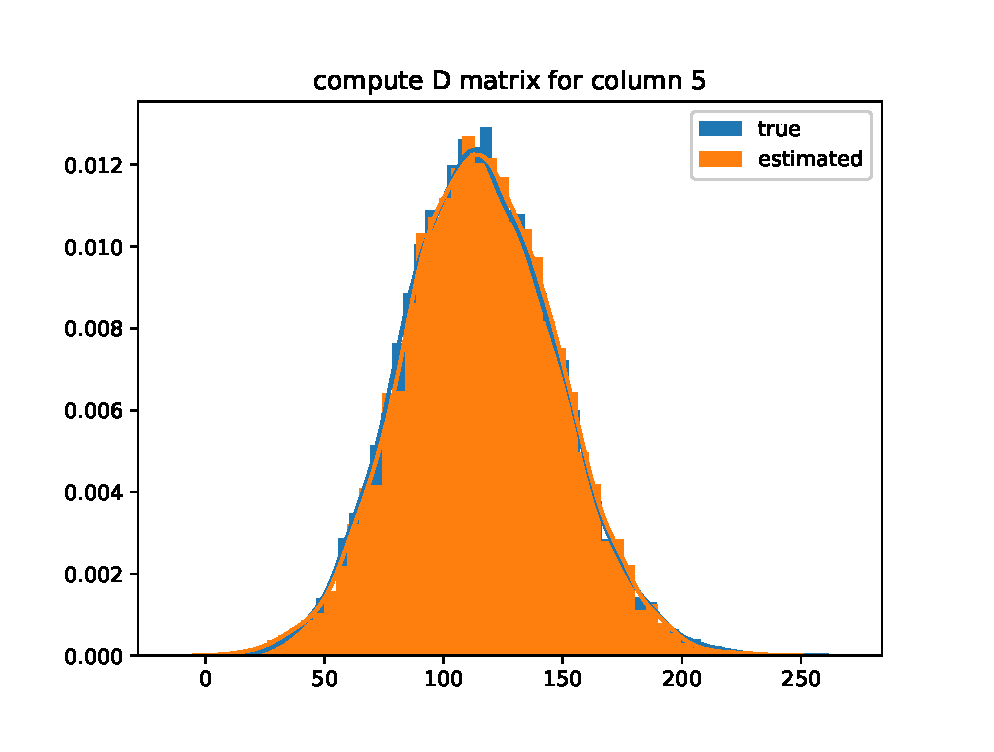
\includegraphics[width=\columnwidth]{d_testing}
\caption{Approximation of product of Gaussians.}
\label{fig:d_testing}
\end{figure}

\begin{figure}[t]
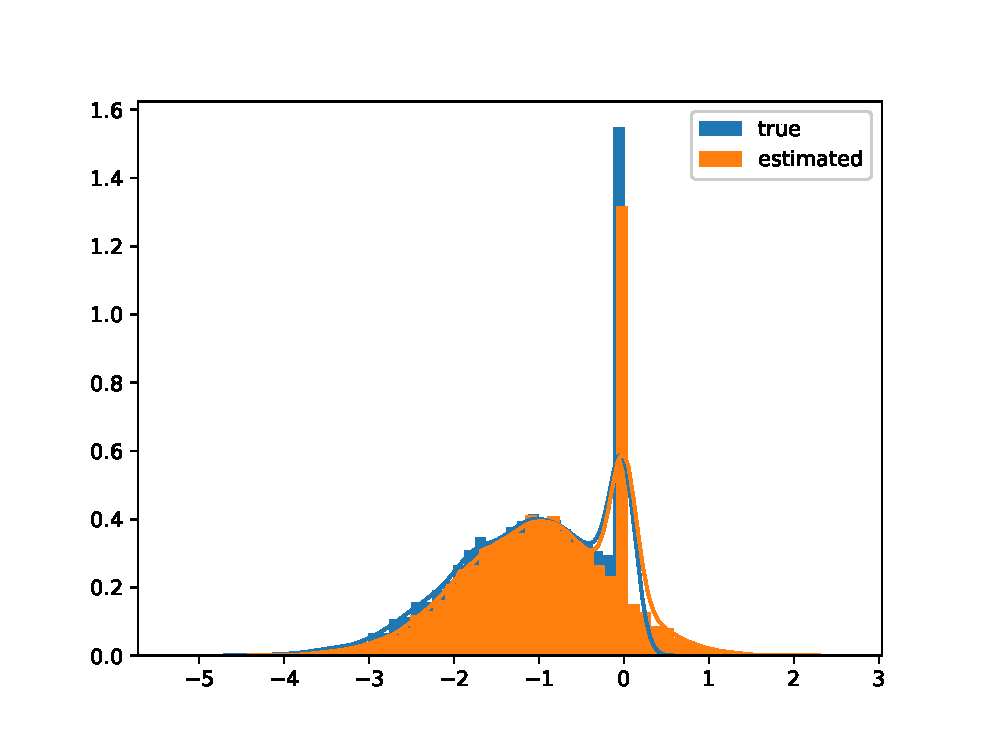
\includegraphics[width=\columnwidth]{z_new_testing}
\caption{Approximation of propagation through soft thresholding}
\label{fig:z_new_testing}
\end{figure}


\section{\uppercase{Backpropagation}}
\label{sec:backpropagation}

The exact posterior (\ref{eq:posterior}) is approximated with a factorised distribution
\begin{align}
\label{eq:approximating_dsitribution}
\begin{split}
q(\mathbf{W}, \mathbf{S}, \gamma, \eta) &= \prod_{d=1}^D\prod_{k=1}^K \mathcal{N}(w_{dk} | m^w_{dk}, v^w_{dk}) \\
&\times \prod_{d'=1}^D\prod_{d''=1}^D \mathcal{N}(s_{d'd''} | m^s_{d'd''}, v^s_{d'd''}) \\
&\times \text{Gam}(\gamma; a^\gamma, b^\gamma) \text{Gam}(\eta; a^\eta, b^\eta) 
\end{split}
\end{align}

For Bayesian inference we expand the probabilistic backpropagation algorithm~\citep{hernandez2015probabilistic} for computing parameter updates. It is based on assumed density filtering (ADF) and expectation propagation (EP) and allows to update parameters of the distributions based on the derivative of the logarithm of a normalisation constant. ADF is based on iterative incorporation of factors from the true posterior $p$ (\ref{eq:posterior}) into the factorised approximating distribution $q$ (\ref{eq:approximating_dsitribution}), whereas in EP factors in the $q$ are iteratively replaced by factors from $p$.

When a factor $p$ is incorporated into $q$, $q$ as a function of Gaussian-distributed weights $W$  and $S$ has the following form:
\begin{equation}
q(\cdot) = Z^{-1}f(\cdot)\mathcal{N}(\cdot; m, v)
\end{equation}
where $Z$ is the normalisation constant and $f(\cdot)$ - arbitrary function. 

According to \cite{minka2001thesis}, new parameters of Gaussian distribution for$ \cdot$ can be computed as
\begin{align}
m^{\text{new}} &= m + v \frac{\partial \log Z}{\partial m}, \\
v^{\text{new}} &= v - v^2\left[ \left(\frac{\partial \log Z}{\partial m}\right)^2 - 2 \frac{\partial \log Z}{\partial v}\right]
\end{align}

Then to find new values of $W$, $S$ we need to compute the $Z$ every time when the factor of the true posterior is incorporated in $q$.

\subsection{\uppercase{Likelihood}}

With the likelihood factors~(\ref{eq:likelihood}) of the true posterior we employ the ADF approach and iteratively incorporate them into the approximating distribution $q$. The normalisation constant of the approximating distribution $q$ with the likelihood term for the data point $n$ incorporated can be computed as follows (to simplify notation the superscript $(n)$ is omitted)
\begin{align}
\label{eq:Z}
\begin{split}
Z = \int \prod_{d=1}^{D} \big[&\mathcal{N}(\beta_d | f(\mathbf{y} ; \mathbf{S}, \mathbf{W}, \lambda), \gamma^{-1}) \\
 &q(\mathbf{W}, \mathbf{S}, \gamma, \eta)\big] \mathrm{d}\mathbf{W} \mathrm{d}\mathbf{S} \mathrm{d}\gamma \mathrm{d}\eta
 \end{split}
\end{align}
We sample $\mathbf{W}$, $\mathbf{S}$ from $q$ and get $\widehat{\boldsymbol\beta}_L = f(\mathbf{y} ; \mathbf{S}, \mathbf{W}, \lambda)$, that is the output from the network and approximated with the spike and slab distribution with parameters $\boldsymbol\omega^{\widehat{\boldsymbol\beta}_L}$, $\mathbf{m}^{\widehat{\boldsymbol\beta}_L}$, and $\mathbf{v}^{\widehat{\boldsymbol\beta}_L}$
\begin{align}
&Z \approx \int \prod_{d=1}^{D} \big[\mathcal{N}(\beta_d | [\widehat{\boldsymbol\beta}_L]_d, \gamma^{-1}) \nonumber \\
&\times (\omega^{\widehat{\boldsymbol\beta}_L}_d \delta_0([\widehat{\boldsymbol\beta}_L]_d) + (1 - \omega^{\widehat{\boldsymbol\beta}_L}_d)\mathcal{N}([\widehat{\boldsymbol\beta}_L]_d | m^{\widehat{\boldsymbol\beta}_L}_d, v^{\widehat{\boldsymbol\beta}_L}_d)) \nonumber\\
&\times \text{Gam} (\gamma_d; \alpha^\gamma, \beta^\gamma)\big]\mathrm{d}\widehat{\boldsymbol\beta}_L \mathrm{d}\gamma  \nonumber\\
&= \prod_{d=1}^{D} \Big[\omega^{\widehat{\boldsymbol\beta}_L}_d \int \big[\mathcal{N}(\beta_d | [\widehat{\boldsymbol\beta}_L]_d, \gamma^{-1})  \delta_0([\widehat{\boldsymbol\beta}_L]_d) \nonumber \\
&\times \text{Gam} (\gamma; \alpha^\gamma, \beta^\gamma)\big]\mathrm{d}[\widehat{\boldsymbol\beta}_L]_d \mathrm{d}\gamma  \nonumber\\
& + (1 - \omega^{\widehat{\boldsymbol\beta}_L}_d)\int \big[\mathcal{N}(\beta_d | [\widehat{\boldsymbol\beta}_L]_d, \gamma^{-1})\nonumber\\
&\times \mathcal{N}([\widehat{\boldsymbol\beta}_L]_d | m^{\widehat{\boldsymbol\beta}_L}_d, v^{\widehat{\boldsymbol\beta}_L}_d)) \text{Gam} (\gamma; \alpha^\gamma, \beta^\gamma)\big]\mathrm{d}[\widehat{\boldsymbol\beta}_L]_d \mathrm{d}\gamma\Big]  \nonumber\\
& = \prod_{d=1}^{D} \Big[\omega^{\widehat{\boldsymbol\beta}_L}_d \int \mathcal{N}(\beta_d | 0, \gamma^{-1})  \text{Gam} (\gamma; \alpha^\gamma, \beta^\gamma) d\gamma  \nonumber\\
& + (1 - \omega^{\widehat{\boldsymbol\beta}_L}_d)\int \big[\mathcal{T}(\beta_d | [\widehat{\boldsymbol\beta}_L]_d, \frac{\beta^\gamma}{\alpha^\gamma}, 2\alpha^\gamma)  \nonumber\\
&\times \mathcal{N}([\mathbf{\widehat{\boldsymbol\beta}_L}]_d| m^{\widehat{\boldsymbol\beta}_L}_d, v^{\widehat{\boldsymbol\beta}_L}_d))\big] \mathrm{d}[\widehat{\boldsymbol\beta}_L]_d\Big]  \nonumber\\
& \approx \prod_{d=1}^D \Big[\omega^{\widehat{\boldsymbol\beta}_L}_d  \mathcal{T}(\beta_d | 0, \frac{\beta^\gamma}{\alpha^\gamma}, 2\alpha^\gamma) \nonumber \\ 
\label{eq:Z_approx}
&+ (1 - \omega^{\widehat{\boldsymbol\beta}_L}_d)\mathcal{N}(\beta_d | m^{\widehat{\boldsymbol\beta}_L}_d, \frac{\beta^\gamma}{\alpha^\gamma - 1} + v^{\widehat{\boldsymbol\beta}_L})\Big]
\end{align}

The Student t density can be parametrised in different ways. In this paper the following parametrisation is used 
\begin{equation}
\mathcal{T}(x; \mu, \beta, \nu) = \frac{\Gamma\left(\frac{\nu + 1}{2}\right)}{\Gamma\left(\frac{\nu}{2}\right)\sqrt{\pi \nu \beta}} \left(1 + \frac{(x - \mu)^2}{\nu\beta}\right)^{-\frac{\nu + 1}{2}}
\end{equation}
where $\Gamma(\cdot)$ denotes the Gamma function.

Parameters of the approximating posterior distribution are then updated with the derivates of this normalisation constant. [ADD ABOUT RECURRENT ESTIMATION]

\subsection{\uppercase{Prior}}
Prior factors from $p$ (\ref{eq:ws}, \ref{eq:gamma_eta}) are incorporated into $q$ with the EP algorithm, i.e. they replace the corresponding approximating factors from $q$ and then $q$ is updated to minimise its KL divergence with $q$ that has the true factor incorporated.

\subsection{\uppercase{Hyperparameter optimisation}}
The only hyperparameter in the proposed Bayesian \textsc{lista} is the shrinkage parameter $\lambda$. It can be optimised using the Type II maximum likelihood procedure. The Type II likelihood, i.e. the evidence $p(\boldsymbol\beta | \mathbf{y}, \lambda)$, of the Bayesian \textsc{lista} is equal to the normalisation constant $Z$ (\ref{eq:Z}) computed for the whole training dataset $\boldsymbol\beta$. Given the approximation~(\ref{eq:Z_approx}) the optimal hyperparameter $\lambda$ can be found by a gradient-based optimiser.

\section{\uppercase{Experiments}}
\label{sec:experiments}
The proposed Bayesian \textsc{lista} is evaluated in the context of the sparse coding problem with an undercomplete dictionary, where the number of measurements $K$ is much smaller than the dimensionality of the vector $\boldsymbol\beta$.

We compare the proposed Bayesian \textsc{lista} with the classical \textsc{lista}~\citep{gregor2010learning} in terms of the predictive accuracy. As baselines we also use \textsc{ista} \citep{daubechies2004iterative} and Fast \textsc{ista} (\textsc{fista}) \citep{beck2009fast}. \textsc{fista} adds the momentum to \textsc{ista} and improves its convergence speed. We limit the number of iterations in these algorithms with $L$ that is the same as the number of layers in Bayesian \textsc{lista} and \textsc{lista}. To measure the performance of the algorithms the normalised mean square error(\textsc{nmse}) and F measure are used. \textsc{nmse} for a batch of data $\{\boldsymbol\beta^{(n)}\}_{n=1}^{N}$ and estimators $\{\widehat{\boldsymbol\beta}^{(n)}\}_{n=1}^{N}$ is computed as
\begin{equation}
\text{\textsc{nmse}} = \frac{1}{N}\sum\limits_{n=1}^N\sqrt{\frac{\sum\limits_{d=1}^D\left(\widehat{\beta}_{d}^{(n)} - \beta_d^{(n)}\right)^2}{\sum\limits_{d=1}^D\left(\beta_{d}^{(n)}\right)^2}}
\end{equation}
In sparse coding it is usually more important to obtain the correct locations of spikes (i.e zeros) and slabs (i.e. non-zeros) in the estimator than to minimise \textsc{nmse}. The problem is therefore viewed as a skewed two-class classification problem where the number of spikes is higher than the number of slabs. F measure is used to evaluate the accuracy of such problems. 
F measure is computed as the harmonic mean of precision and recall
\begin{equation}
\text{F measure} = 2\dfrac{\text{precision}\cdot\text{recall}}{\text{precision} + \text{recall}}
\end{equation} 
where precision is the fraction of estimated slab locations that are correct, recall is the fraction of true slab locations among all predicted slab locations.
We demonstrate the performance on small datasets to highlight that the proposed algorithm can infer accurate predictions when the dataset size is not sufficient for \textsc{lista} to learn. 

\subsection{\uppercase{Predictive performance on synthetic data}}
First, the predictive performance of the proposed Bayesian \textsc{lista} is analysed on synthetic data. We generate $N_\text{train}=500$ sparse coefficients vectors $\boldsymbol\beta_n$ each of size $D = 100$. Coefficients $\boldsymbol\beta$ are generated from the spike and slab distribution with truncated slab: each component of $\beta_{nd}$ is zero with probability $0.8$ or is from standard Gaussian distribution without interval $(-0.1, 0.1)$ with probability $0.2$. Truncation of the zeros allows to remove from support pattern values with insignificant contributions \citep{xin2016maximal}. To simulate sparse observations, we have generated the random Gaussian design matrix $\mathbf{X} \in \mathbb{R}^{K \times D}$.  The observations are generated according to the \ref{eq:regression_problem} with zero-mean Gaussian noise with standard deviation $0.5$. $\lambda$ is assumed fixed as $0.1$.

In the Figure \ref{fig:number_of_layers_synthetic} prediction performance for different number of layers $L$ is presented. The observation size is set as $K=50$. In both experiments the performance of the Bayesian \textsc{lista} is better than the performance of \textsc{lista}. Although the baseline \textsc{ista} and \textsc{fista} show better performance in terms of F measure, Bayesian \textsc{lista} has lower \textsc{nmse}.

In the Figure \ref{fig:unsersampling_synthetic} prediction performance for different observation sizes $K$ is presented. The number of layers is set as $L=4$ which is the value of the poorest performance of Bayesian \textsc{lista} according to the previous experiment. Bayesian \textsc{lista} provides better results than {lista} for $K \ge 30$ and better results than other algorithms for $K \ge 70$.

\begin{figure}[t]
\centering
%\subfloat[\textsc{nmse} on train]{\includegraphics[width=0.5\columnwidth]{graphics/synthetic_number_of_layers/nmse_train}}
%~
\subfloat[\textsc{nmse} on validation]{\includegraphics[width=0.5\columnwidth]{graphics/synthetic_number_of_layers/nmse_validation}}
%\subfloat[F measure on train]{\includegraphics[width=0.5\columnwidth]{graphics/synthetic_number_of_layers/f_measure_train}}
%~
\subfloat[F measure on validation]{\includegraphics[width=0.5\columnwidth]{graphics/synthetic_number_of_layers/f_measure_validation}}
\caption{Predictive accuracy on different number of layers (for neural networks) or iterations (for baselines) on the synthetic data}
\label{fig:number_of_layers_synthetic}
\end{figure}

\begin{figure}[t]
\centering
%\subfloat[\textsc{nmse} on train]{\includegraphics[width=0.5\columnwidth]{graphics/synthetic_undersampling/nmse_train}}
%~
\subfloat[\textsc{nmse} on validation]{\includegraphics[width=0.5\columnwidth]{graphics/synthetic_undersampling/nmse_validation}}
%\subfloat[F measure on train]{\includegraphics[width=0.5\columnwidth]{graphics/synthetic_undersampling/f_measure_train}}
%~
\subfloat[F measure on validation]{\includegraphics[width=0.5\columnwidth]{graphics/synthetic_undersampling/f_measure_validation}}
\caption{Predictive performance on different size of observations on the synthetic data}
\label{fig:unsersampling_synthetic}
\end{figure}

%We compare two versions of the proposed Bayesian LISTA: with shared weight matrices and with individual matrices at each layer --- and LISTA.

%The NMSE is presented in figure \ref{fig:validation_synthetic}.
%\begin{figure}[t]
%\includegraphics[width=\columnwidth]{loss_synthetic}
%\caption{Validation NMSE on synthetic data}
%\label{fig:validation_synthetic}
%\end{figure}

\subsection{\uppercase{Predictive performance on mnist data}}
Here we evaluate the proposed Bayesian \textsc{lista} in terms of predictive performance on the \textsc{mnist} dataset \citep{lecun1998gradient}. The dataset contains images of handwritten digits of size $28 \times 28 = 784$. The design matrix $\mathbf{X}$ is learned on 5000 images with the minibatch online algorithm \citep{mairal2009online}. The resulting size of $\mathbf{X}$ is $K \times 784$. Then we generate observations as $\mathbf{y} = \mathbf{X}\boldsymbol\beta$, where $\boldsymbol\beta$ are images converted to vectors. We use randomly selected $100$ images for training and $100$ for validation. $\lambda$ is assumed fixed as $0.1$.

Figures \ref{fig:mnist_100} and \ref{fig:mnist_250} present quality on the validation set with dictionaries of size $100$ and $250$.  When $K=100$ Bayesian \textsc{lista} shows better performance that other algorithms and on $K=250$ it  converges to similar values as \textsc{lista}.

Proposed Bayesian \textsc{lista} networks estimate posterior distribution for $\boldsymbol\beta$. Figure \ref{fig:posterior_samples} shows samples from the posterior for one of the validation data points and Figure \ref{fig:posterior_distribution} shows the parameters of this posterior.

\begin{figure}[t]
\centering
%\subfloat[\textsc{nmse} on train]{\includegraphics[width=0.5\columnwidth]{graphics/mnist/100_normalised_nmse_train}}
%~
\subfloat[\textsc{nmse} on validation]{\includegraphics[width=0.5\columnwidth]{graphics/mnist/100_normalised_nmse_valid}}
%\subfloat[F measure on train]{\includegraphics[width=0.5\columnwidth]{graphics/mnist/100_normalised_f_measure_train}}
%~
\subfloat[F measure on validation]{\includegraphics[width=0.5\columnwidth]{graphics/mnist/100_normalised_f_measure_valid}}
\caption{Predictive performance on number of iterations on the \textsc{mnist} data with dictionary size $K = 100$}
\label{fig:mnist_100}
\end{figure}

\begin{figure}[t]
\centering
%\subfloat[\textsc{nmse} on train]{\includegraphics[width=0.5\columnwidth]{graphics/mnist/250_normalised_nmse_train}}
%~
\subfloat[\textsc{nmse} on validation]{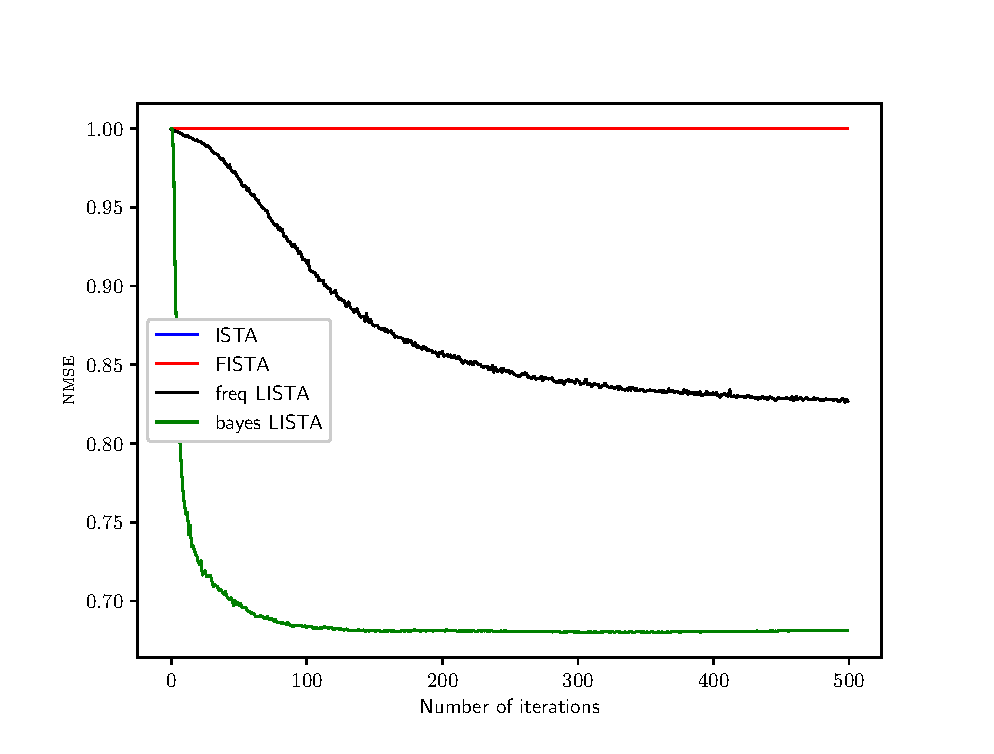
\includegraphics[width=0.5\columnwidth]{graphics/mnist/250_normalised_nmse_valid}}
%\subfloat[F measure on train]{\includegraphics[width=0.5\columnwidth]{graphics/mnist/250_normalised_f_measure_train}}
%~
\subfloat[F measure on validation]{\includegraphics[width=0.5\columnwidth]{graphics/mnist/250_normalised_f_measure_valid}}
\caption{Predictive performance on number of iterations on the \textsc{mnist} data with dictionary size $K = 250$}
\label{fig:mnist_250}
\end{figure}

%\begin{figure}[t]
%\includegraphics[width=\columnwidth]{loss}
%\caption{Validation \textsc{nmse}}
%\label{fig:validation}
%\end{figure}
\begin{figure}[t]
\centering
\subfloat[$\beta$ posterior mean]{\includegraphics[width=0.33\columnwidth]{posterior_mean}}~
\subfloat[$\beta$ posterior std]{\includegraphics[width=0.33\columnwidth]{posterior_std}}~
\subfloat[$\beta$ posterior spike indicator]{\includegraphics[width=0.33\columnwidth]{posterior_spike_indicator}}
\caption{Posterior parameters for an image of digit 7.}
\label{fig:posterior_distribution}
\end{figure}
\begin{figure}[t]
\centering
\subfloat[]{\includegraphics[width=0.33\columnwidth]{posterior_sample_0}}~
\subfloat[]{\includegraphics[width=0.33\columnwidth]{posterior_sample_1}}~
\subfloat[]{\includegraphics[width=0.33\columnwidth]{posterior_sample_2}}
\caption{Samples from the posterior for an image of digit 7.}
\label{fig:posterior_samples}
\end{figure}

\subsection{\uppercase{Active learning}}
To demonstrate the potential scenario that can benefit from uncertainty estimates of the Bayesian \textsc{lista} we consider the active learning example \citep{settles.tr09}. Active learning area researches ways to select new training subsets to reduce total number of required supervision. One of the approaches for active learning is uncertainty sampling when the data with the least certain predictions is used for training. The uncertainty can be measured with entropy or variance. In our example no closed form for entropy of spike and slab exist, therefore we use variance from lemma \ref{thm:moments_spsl} as a measure of uncertainty.

The data in this example is the same \textsc{mnist} dataset with learnt dictionary of size $K=100$. It is divided into train data of size $50$, pool data of size $500$,  and test data of size $100$. The algorithm learns on the train data for $50$ iterations. After that, the Bayesian \textsc{lista} algorithm iteratively estimates the variance of the predictions on the pool data, selects the element with the maximum variance, moves it from pool set to the training set and runs additional training iteration. Overall, $10$ pool iterations are performed.

The performance on the actively updated train data is compared with the performance on the randomly updated train data, when at every iteration the random element is moved from pool set to train set. Both algorithms of new data sampling were run with $20$ random seeds and their performance was averaged. Figure \ref{fig:active_learning_mnist} demonstrates their performance.The uncertainty sampling has some advantage compared to random sampling, this means that the posterior variance is adequately estimated.
\begin{figure}[t]
\centering
\subfloat[\textsc{nmse}]{\includegraphics[width=0.5\columnwidth]{graphics/active_mnist/nmse_validation}}%
\subfloat[F measure]{\includegraphics[width=0.5\columnwidth]{graphics/active_mnist/f_measure_validation}}
\caption{Performance in the active learning experiment on the \textsc{mnist} data. }
\label{fig:active_learning_mnist}
\end{figure}

\section{\uppercase{Discussion}}
\label{sec:discussion}
To the best of our knowledge, this is the first implementation of Bayesian deep sparse coding algorithm. Although there are works on Bayesian sparsity in context of neural networks \citep{he2017bayesian}, they are not the Bayesian neural networks in the same sense as Bayesian \textsc{lista} but rather the interpretation of the sparse Bayesian  learning algorithm as the long short-term memory network. We find not only correct predictions but also useful posterior estimates for the predictions that show how the model is confident in its decisions. 

%The inference is based on the expectation propagation algorithm and though it is not suited for distributed inference, stochastic variant of assumed density filtering can potentially be used \citep{li2015stochastic}. This would allow the proposed approach to scale.

The \textsc{lista}-based algorithms can be applied for the sparse coding problem with both overcomplete dictionaries as in the original paper \citep{gregor2010learning}, and undercomplete dictionaries \citep{borgerding2017amp}. Though this paper presents only results with undercomplete dictionaries, this is not the limitation of the proposed method and it can be used for overcomplete dictionaries in a similar manner.

\section{\uppercase{Conclusions and future work}}
\label{sec:conclusions}
We have presented the new method for propagating the uncertainty through the soft thresholding function. %To achieve this goal 
We have approximated the outputs of the function with a spike and slab distribution, and we have shown that this distribution can stay within the same family after linear transformation with Gaussian weights and inputs of a neural network. This allowed us to propose the Bayesian \textsc{lista} network and efficient inference algorithm that learns the distributions of the weights and makes the uncertainty estimates of the outputs. The forward propagation in the algorithm is based on the proposed uncertainty propagation method, the backward propagation is based on the probabilistic backpropagation method, that was remarkably expanded to account for multidimensionality of inputs and outputs, likelihood of the Bayesian \textsc{lista} and its recurrent nature.

Experiments on the synthetic and \textsc{mnist} datasets demonstrate that the proposed algorithm preserves the predictive accuracy of non-Bayesian methods while also providing posterior estimates. We also show that when the training data is very small the proposed algorithm significantly outperforms the classical \textsc{lista} in terms of predictive accuracy. Experiments on active learning demonstrate that the proposed Baysian \textsc{lista} gives accurate posterior estimates that can be used for selection of a next data point where a label should be obtain for. 

The shrinkage parameter $\lambda$ is currently treated as a deterministic hyperparameter for the Baysian \textsc{lista}. In future we plan to incorporate it into the model treating it as a random variable. For this we need to extend both the uncertainty propagation method to include uncertainty of $\lambda$ and the probabilistic backpropagation algorithm to estimate its posterior. We will study stochastic expectation propagation applicability in order to replace ADF that may improve further the quality of posterior estimates~\citep{li2015stochastic}.    
\bibliography{bibliography}
\bibliographystyle{icml2018}

\end{document}
